\section{ZX-calculus and Pauli webs}\label{sec:zx-calculus-and-pauli-webs}

Throughout this work we've used the \textit{ZX-calculus} and \textit{Pauli webs} in the figures.
Here we give a very quick explainer of some of our notation, and give references for the reader interested in learning more.
The ZX-calculus is a graphical language for reasoning about quantum mechanics.
Two great introductions are \Ccite{vandewetering2020zxcalculusworkingquantumcomputer,KissingerWetering2024Book}.
A ZX-diagram consists of green and red \textit{spiders} with input and output legs, which one can think of as just very good notation for families of linear maps
\begin{equation}\label{eq:spiders_defn}
    \begin{aligned}
        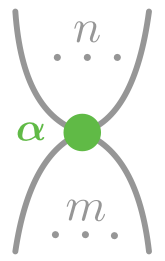
\includegraphics[height=50pt,valign=c]{figures/appendix/zx/Z-spider}
        &\coloneqq \ket{0}^{\otimes n}\bra{0}^{\otimes m} + e^{i\alpha}\ket{1}^{\otimes n}\bra{1}^{\otimes m}, \\
        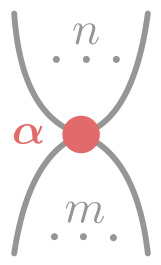
\includegraphics[height=50pt,valign=c]{figures/appendix/zx/X-spider}
        &\coloneqq \ket{+}^{\otimes n}\bra{+}^{\otimes m} + e^{i\alpha}\ket{-}^{\otimes n}\bra{-}^{\otimes m}.
    \end{aligned}
\end{equation}
These spider legs can be connected together, corresponding to composition of linear maps, and spiders can be placed alongside each other, corresponding to taking tensor products.
In this work, we additionally used the shorthands
\begin{equation}\label{eq:zx_shorthands}
    
\includegraphics[height=55pt, valign=c]{figures/appendix/zx/Hadamard} \coloneqq
    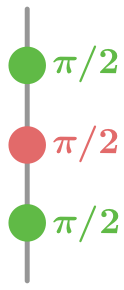
\includegraphics[height=55pt, valign=c]{figures/appendix/zx/Hadamard_decomposed} ,\qqquad
    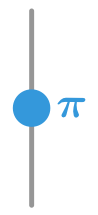
\includegraphics[height=40pt, valign=c]{figures/appendix/zx/Y_gate} \coloneqq
    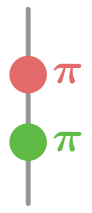
\includegraphics[height=40pt, valign=c]{figures/appendix/zx/ZX_gate} ,\qqquad
    
\includegraphics[height=40pt, valign=c]{figures/appendix/zx/plus_gate} \coloneqq
    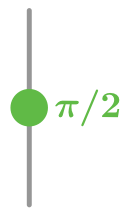
\includegraphics[height=40pt, valign=c]{figures/appendix/zx/pi_over_2_Z_gate} ,\qqquad
    
\includegraphics[height=40pt, valign=c]{figures/appendix/zx/minus_Z_gate} \coloneqq
    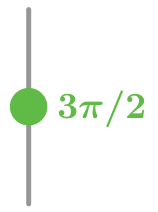
\includegraphics[height=40pt, valign=c]{figures/appendix/zx/3pi_over_2_Z_gate}.
\end{equation}
We also got a bit cheeky and drew some spiders/shorthands right on top of each other, hiding the connecting wire
\begin{equation}\label{eq:compressed_ZZ_measurement}
    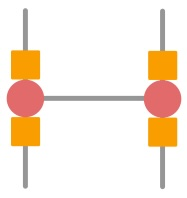
\includegraphics[height=40pt, valign=c]{figures/appendix/zx/ZZ_measurement_close_together} \quad = \quad
    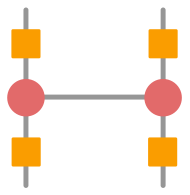
\includegraphics[height=40pt, valign=c]{figures/appendix/zx/ZZ_measurement_spaced_out}.
\end{equation}
We continued to be cheeky when we said that certain diagrams correspond to measurements of $X \otimes X$, $Y \otimes Y$ and $Z \otimes Z$ in \Cref{fig:schedules_XYZ_and_CSS}.
In reality, the diagrams there are equal (up to positive scalar) to the projections onto the $+1$ eigenspaces of $X \otimes X$, $Y \otimes Y$ and $Z \otimes Z$ respectively.
In other words, it's as if we're assuming throughout that we always get measurement outcome $+1$, despite many of these measurements being totally random.
It turns out that for reasoning about QEC protocols, we can get away with this, as explained (very briefly!) in \Ccite[Appendix G]{Townsend_Teague_2023}.

ZX-diagrams can additionally be annotated with \textit{Pauli webs}.
One can think of these as describing how Pauli gates commute with individual spiders in a ZX-diagram.
A nice introduction to them can be found in \Ccite{rodatz2024floquetifyingstabilisercodesdistancepreserving}.
The important part with respect to making sense of the figures in this work is that `closed' Pauli webs (ones in which no overall input or output leg of the ZX-diagram is highlighted) correspond to detectors.
Whether a set of Pauli errors violates a detector can then be seen graphically -- this happens if and only if there are an odd number of edges that are highlighted in a colour other than the colour of the Pauli error that sits on it.
For example, the following sets of Pauli errors on consecutive $Z \otimes Z$ measurements violate the corresponding detector
\begin{equation}\label{eq:ZZ_detector_violated}
    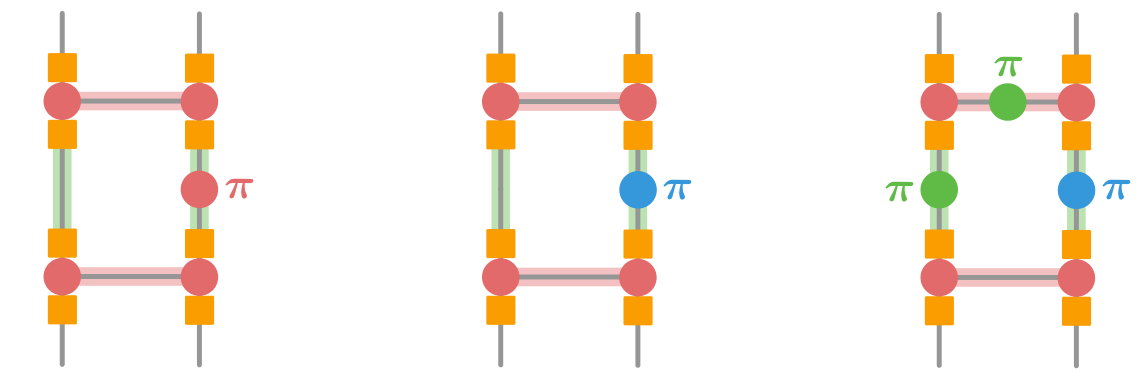
\includegraphics[height=70pt, valign=c]{figures/appendix/zx/ZZ_measurements_violating_errors}.
\end{equation}
On the other hand, these sets of Pauli errors don't violate it
\begin{equation}\label{eq:ZZ_detector_not_violated}
    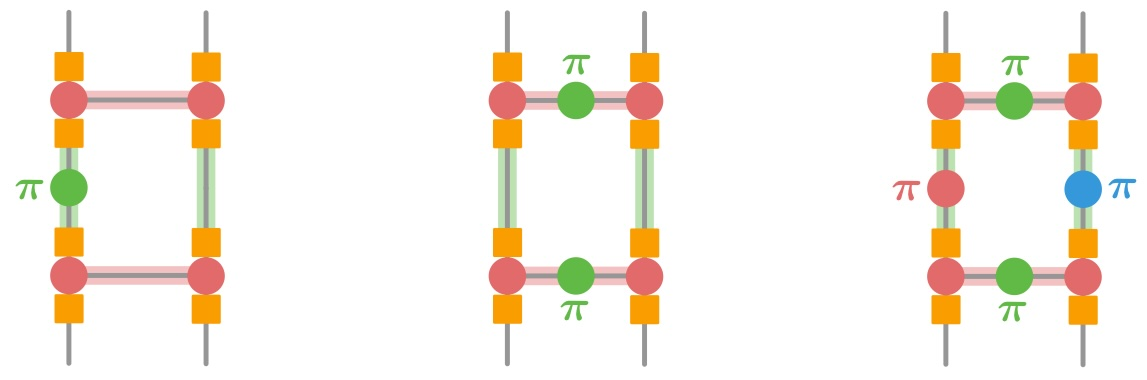
\includegraphics[height=70pt, valign=c]{figures/appendix/zx/ZZ_measurements_non_violating_errors}.
\end{equation}
So given a closed Pauli web, one can read off which measurements make up the corresponding detector, and which types of Pauli errors this detector can detect at different time steps.
Namely, since measurement errors correspond to 
green two-legged 
$\pi$-spiders 
on `horizontal' 
wires (\Cref{fig:phenom_error_examples}), the corresponding measurement is only included in a detector 
if this wire is 
highlighted red or blue.
For example, in \Cref{fig:detectors_XYZ_and_CSS} we can now read off that the detector in the $X^1 Y^1 Z^1$ honeycomb code consists of twelve detectors, while the detector in the $X^1 Z^1$ honeycomb code consists of only six.
For more details, see \Ccite{rodatz2024floquetifyingstabilisercodesdistancepreserving}, or the handful of other works that make use of Pauli webs~\cite{bombin2024unifying,McEwen_2023,wan2025pauliwebyranglestate,delafuente2024xyzrubycodemaking, Townsend_Teague_2023}.
